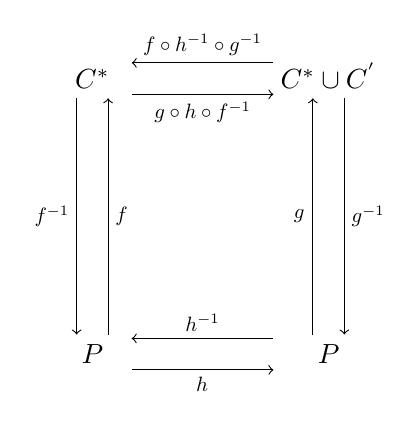
\begin{tikzpicture}
\def\a{1.5} \def\b{3}
\coordinate (A) at (-\a,0);
\coordinate (B) at (\a,0) ;
\coordinate (C) at (\a,-\b) ;
\coordinate (D) at (-\a,-\b) ;
\node[above] at (A) {$C^{*}$}  ;   
\node[above] at (B)  {$C^{*}\cup C^{'}$};
\node[below] at (C) {$\mathbb{P}$};
\node[below] at (D) {$\mathbb{P}$};
\coordinate (E) at  (-1,-3.25) {};
\coordinate (F) at  (0.8,-3.25) {};
\coordinate (G) at  (-1,0.2) {};
\coordinate (H) at  (0.8,0.2) {};
\begin{scope}[nodes={midway,scale=.75}, shift = {(-0.2,0)}]
\draw[->] (-\a,0)--(-\a,-\b)  node[left]{$f^{-1}$};
\draw[<- ](B) (\a,0)--(\a,-\b) node[left]{$g^{}$};
\end{scope}
\begin{scope}[nodes={midway,scale=.75}, shift = {(0.2,0)}]
\draw[<-] (-\a,0)--(-\a,-\b)  node[right]{$f^{}$};
\draw[->] (B) (\a,0)--(\a,-\b) node[right]{$g^{-1}$};
\end{scope}

\begin{scope}[nodes={midway,scale=.75}, shift = {(0.,0.2)}]
\draw[<-] (-1,-3.25)-- (0.8,-3.25) node[above]{$h^{-1}$};
\end{scope}
\begin{scope}[nodes={midway,scale=.75}, shift = {(0.,-0.2)}]
\draw[->] (-1,-3.25)-- (0.8,-3.25) node[below]{$h^{}$};
\end{scope}

\begin{scope}[nodes={midway,scale=.75}, shift = {(0.,0.2)}]
\draw[<-] (-1,.25)-- (0.8,.25) node[above]{$f\circ h^{-1}\circ g^{-1}$};
\end{scope}
\begin{scope}[nodes={midway,scale=.75}, shift = {(0.,-0.2)}]
\draw[->] (-1,.25)-- (0.8,.25) node[below]{$g\circ h\circ f^{-1}$};
\end{scope}
\end{tikzpicture} 